\documentclass[border=0.8ex,svgnames,tikz]{standalone}
\usepackage{amsmath,mathtools}
\usepackage{fontspec}
\setmainfont{Source Serif 4}
\setsansfont{Source Sans 3}
\setmonofont{Source Code Pro}
\usetikzlibrary{positioning}
\begin{document}
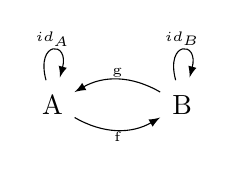
\begin{tikzpicture}[
  every node/.style={circle,minimum size=1.8em,inner sep=0.5ex},
  every path/.style={auto,draw,>=latex},
  label node/.style={sloped,inner sep=-0.5ex,minimum size=1ex,font=\tiny},
  ]
  \node(A){A};
  \node[right=of A](B){B};
  \path[->]
  (A) edge[bend right] node[below,label node]{f} (B)
  (B) edge[bend right] node[above,label node]{g} (A)
  (A) edge[loop above] node[label node]{\(id_{A}\)} ()
  (B) edge[loop above] node[label node]{\(id_{B}\)} ();
\end{tikzpicture}
\end{document}
